\documentclass[11pt]{article}
% Shared preamble for the lecture notes
\usepackage[T1]{fontenc}
\usepackage[utf8]{inputenc}
\usepackage[a4paper,margin=2.4cm]{geometry}
\usepackage{amsmath,amssymb,amsthm,mathtools}
\usepackage{bm}
\usepackage{xcolor}
\usepackage{enumitem}
\usepackage{tikz}
\usetikzlibrary{arrows.meta,positioning,calc}
\usepackage{pgfplots}
\pgfplotsset{compat=1.18}
\usepgfplotslibrary{groupplots}
\usepackage[american]{circuitikz}
\usepackage{microtype}
\usepackage[colorlinks=true,linkcolor=accent,urlcolor=accent,citecolor=accent]{hyperref}
\usepackage{fancyhdr}

\definecolor{accent}{HTML}{B4126B}
\definecolor{accent2}{HTML}{0E7C86}
\definecolor{rule}{HTML}{C9C9D6}

\theoremstyle{definition}
\newtheorem{definition}{Definition}[section]
\newtheorem{example}{Example}[section]
\theoremstyle{plain}
\newtheorem{theorem}{Theorem}[section]
\newtheorem{proposition}[theorem]{Proposition}
\newtheorem{lemma}[theorem]{Lemma}
\newtheorem{corollary}[theorem]{Corollary}
\theoremstyle{remark}
\newtheorem*{remark}{Remark}

% handy macros
\newcommand{\dd}{\mathrm{d}}
\newcommand{\E}{\mathbb{E}}
\newcommand{\R}{\mathbb{R}}
\newcommand{\Var}{\operatorname{Var}}
\newcommand{\Cov}{\operatorname{Cov}}
\newcommand{\KL}{D_{\mathrm{KL}}}
\renewcommand{\vec}[1]{\bm{#1}}
\DeclarePairedDelimiter{\abs}{\lvert}{\rvert}
\DeclarePairedDelimiter{\norm}{\lVert}{\rVert}

\pagestyle{fancy}
\fancyhf{}
\renewcommand{\headrulewidth}{0.4pt}
\fancyhead[L]{\small\itshape Information Theory \& Neural Modeling}
\fancyhead[R]{\small M.\ Vissani}
\fancyfoot[C]{\small\thepage}

% title block
\newcommand{\lectitle}[3]{%
  \begin{center}
    {\footnotesize\sffamily\bfseries\color{accent} GRADUATE LECTURE NOTES \quad\textbullet\quad SCUOLA SUPERIORE SANT'ANNA}\\[2pt]
    {\color{rule}\rule{\linewidth}{0.8pt}}\\[8pt]
    {\LARGE\sffamily\bfseries #1}\\[6pt]
    {\large\sffamily #2}\\[6pt]
    {\small Matteo Vissani \quad\textbullet\quad Course: \emph{Information Theory \& Neural Modeling}}\\[6pt]
    {\color{rule}\rule{\linewidth}{0.8pt}}
  \end{center}
  \vspace{0.6em}
}


\begin{document}
\lectitle{Entropy and Mutual Information}{Lecture 2 --- Information-theoretic tools for neural coding}

\begin{abstract}
\noindent We develop Shannon's information theory from the ground up: surprise and entropy, the
asymptotic equipartition property and the source-coding bound, the convexity inequalities (Jensen,
log-sum, Gibbs), joint and conditional entropy, relative entropy, and mutual information with all
its identities. We then go beyond pairwise information to the \emph{multivariate} theory ---
interaction information, total correlation, and the partial information decomposition of a
multi-source channel into \emph{redundant}, \emph{unique}, and \emph{synergistic} components. We
treat continuous variables (differential entropy, maximum-entropy distributions, the Gaussian
channel and water-filling), the data-processing and Fano inequalities, and close with a detailed
application to neural coding: the noise/response decomposition, the direct method and its
finite-sample bias, the Fisher-information lower bound, and synergy and redundancy in neural
populations.
\end{abstract}

\tableofcontents
\vspace{1em}

%==================================================================
\section{Surprise, entropy, and compression}
%==================================================================

Let $X$ be a discrete random variable on an alphabet $\mathcal X$ with pmf $p(x)$. The
\emph{surprise} of an outcome is $h(x)=-\log p(x)$: it is additive over independent events and
decreasing in probability, the only such functional up to a base. With base $2$ the unit is the
\emph{bit}.

\begin{definition}[Entropy]
$\displaystyle H(X)=\E[-\log p(X)]=-\sum_{x}p(x)\log p(x)$, with $0\log0=0$.
\end{definition}

\begin{proposition}[Basic properties]\label{prop:H}
(i) $H(X)\ge0$, with equality iff $X$ is deterministic; (ii) $H(X)\le\log\abs{\mathcal X}$, with
equality iff $X$ is uniform; (iii) $H$ is concave in $p$.
\end{proposition}

\begin{example}[Binary entropy]
$X\sim\mathrm{Bernoulli}(p)$ has $H_2(p)=-p\log p-(1-p)\log(1-p)$, maximal ($1$ bit) at $p=\tfrac12$.
\end{example}

\paragraph{Why entropy is \emph{the} measure: source coding.}
Entropy is not an arbitrary functional; it is the fundamental limit of lossless compression. By
the \textbf{asymptotic equipartition property} (AEP), for i.i.d.\ $X_1,\dots,X_n$,
\begin{equation}
  -\tfrac1n\log p(X_1,\dots,X_n)\xrightarrow{\ \text{a.s.}\ }H(X),
\end{equation}
so the probability mass concentrates on a \emph{typical set} of $\approx 2^{nH(X)}$ roughly
equiprobable sequences. Shannon's source-coding theorem~\cite{shannon1948,coverthomas} then states that the expected code length
$L$ of any uniquely decodable binary code obeys
\begin{equation}
  H(X)\le L < H(X)+1\ \ \text{bits/symbol},
\end{equation}
the lower bound following from the \textbf{Kraft inequality} $\sum_x 2^{-\ell(x)}\le1$ together
with Gibbs' inequality. Entropy is therefore the average number of bits needed to describe $X$.

%==================================================================
\section{Convexity tools}
%==================================================================
\begin{lemma}[Jensen]
For convex $\varphi$, $\E[\varphi(X)]\ge\varphi(\E[X])$ (reversed for concave $\varphi$); equality
iff $X$ is a.s.\ constant or $\varphi$ is affine on the support.
\end{lemma}
\begin{lemma}[Log-sum inequality]
For nonnegative $a_i,b_i$,
$\displaystyle\sum_i a_i\log\frac{a_i}{b_i}\ge\Big(\sum_i a_i\Big)\log\frac{\sum_i a_i}{\sum_i b_i}$,
with equality iff $a_i/b_i$ is constant.
\end{lemma}
These two facts generate essentially every inequality below.

%==================================================================
\section{Joint and conditional entropy}
%==================================================================
For $(X,Y)\sim p(x,y)$ define $H(X,Y)=-\sum_{x,y}p(x,y)\log p(x,y)$ and the conditional entropy
\begin{equation}
  H(Y\mid X)=\sum_x p(x)H(Y\mid X{=}x)=-\sum_{x,y}p(x,y)\log p(y\mid x).
\end{equation}
\begin{theorem}[Chain rule]
$H(X,Y)=H(X)+H(Y\mid X)=H(Y)+H(X\mid Y)$, and more generally
$H(X_1,\dots,X_n)=\sum_{i}H(X_i\mid X_1,\dots,X_{i-1})$.
\end{theorem}
\begin{corollary}[Conditioning reduces entropy; subadditivity]
$H(Y\mid X)\le H(Y)$ and hence $H(X_1,\dots,X_n)\le\sum_i H(X_i)$, with equality iff independent.
\end{corollary}

%==================================================================
\section{Relative entropy (Kullback--Leibler divergence)}
%==================================================================
\begin{definition}
For $p\ll q$, $\displaystyle \KL(p\,\|\,q)=\sum_x p(x)\log\frac{p(x)}{q(x)}=\E_p\!\Big[\log\frac{p(X)}{q(X)}\Big].$
\end{definition}
\begin{theorem}[Gibbs' inequality]\label{thm:gibbs}
$\KL(p\,\|\,q)\ge0$, with equality iff $p=q$.
\end{theorem}
\begin{proof}
By Jensen with the concave $\log$,
$-\KL(p\,\|\,q)=\E_p[\log\frac{q}{p}]\le\log\E_p[\frac{q}{p}]=\log\sum_x q(x)\le0$;
strict concavity forces $p=q$ at equality.
\end{proof}
$\KL$ is the inefficiency (extra bits) of coding for $q$ when the truth is $p$; it is asymmetric
and not a metric, but it dominates the total-variation distance via Pinsker's inequality
$\KL(p\,\|\,q)\ge\frac{1}{2\ln2}\,\norm{p-q}_1^2$.

%==================================================================
\section{Mutual information}\label{sec:mi}
%==================================================================
\begin{definition}
$\displaystyle I(X;Y)=\KL\!\big(p(x,y)\,\|\,p(x)p(y)\big)=\sum_{x,y}p(x,y)\log\frac{p(x,y)}{p(x)p(y)}.$
\end{definition}
\emph{Derivation of the identities.} Start from the definition and split the logarithm using
$p(x,y)=p(x\mid y)\,p(y)$, so $\log\frac{p(x,y)}{p(x)p(y)}=\log p(x\mid y)-\log p(x)$:
\begin{align}
  I(X;Y)&=\sum_{x,y}p(x,y)\Big[\log p(x\mid y)-\log p(x)\Big]\notag\\
  &=\underbrace{-\sum_{x}\Big(\sum_y p(x,y)\Big)\log p(x)}_{=\,H(X)}
   \;-\;\underbrace{\Big(-\sum_{x,y}p(x,y)\log p(x\mid y)\Big)}_{=\,H(X\mid Y)}
   \;=\;H(X)-H(X\mid Y),
\end{align}
where the first sum used $\sum_y p(x,y)=p(x)$. By the symmetry $p(x\mid y)p(y)=p(y\mid x)p(x)$ the
same steps give $H(Y)-H(Y\mid X)$, and substituting the chain rule $H(X\mid Y)=H(X,Y)-H(Y)$ gives
the third form. Hence
\begin{equation}
  \boxed{\;I(X;Y)=H(X)-H(X\mid Y)=H(Y)-H(Y\mid X)=H(X)+H(Y)-H(X,Y).\;}
  \label{eq:mi}
\end{equation}
\begin{theorem}[Properties]\label{thm:I}
(i) $I(X;Y)=I(Y;X)\ge0$, $=0$ iff $X\perp Y$; (ii) $I(X;Y)\le\min\{H(X),H(Y)\}$;
(iii) $I(X;X)=H(X)$.
\end{theorem}

\begin{figure}[h]
\centering
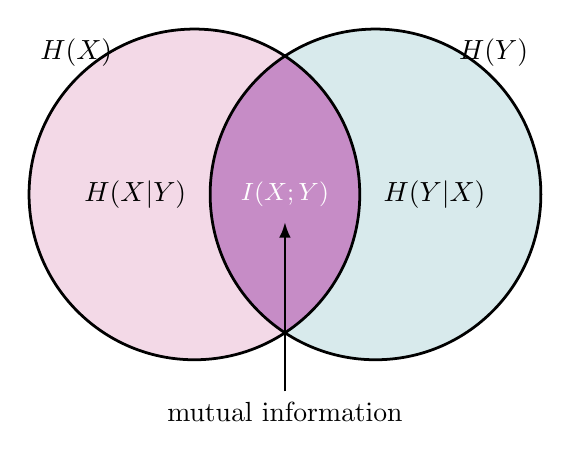
\begin{tikzpicture}[line width=1pt]
  \def\rr{2.1}
  \coordinate (A) at (0,0);
  \coordinate (B) at (2.3,0);
  % X-only region
  \begin{scope}\clip (A) circle(\rr); \fill[accent!16] (A) circle(\rr);\end{scope}
  % Y-only region
  \begin{scope}\clip (B) circle(\rr); \fill[accent2!16] (B) circle(\rr);\end{scope}
  % intersection = mutual information, shaded distinctly
  \begin{scope}\clip (A) circle(\rr); \fill[violet!45] (B) circle(\rr);\end{scope}
  % outlines
  \draw (A) circle(\rr);
  \draw (B) circle(\rr);
  % labels
  \node[font=\bfseries] at (-1.5,1.8) {$H(X)$};
  \node[font=\bfseries] at (3.8,1.8) {$H(Y)$};
  \node at (-0.75,0) {$H(X{\mid}Y)$};
  \node at (3.05,0) {$H(Y{\mid}X)$};
  \node[align=center,font=\small\bfseries,text=white] at (1.15,0) {$I(X;Y)$};
  \draw[-{Latex[length=2mm]}] (1.15,-2.5) node[below]{mutual information} -- (1.15,-0.35);
\end{tikzpicture}
\caption{Information diagram. The shaded lens where the two circles overlap is the mutual
information $I(X;Y)$; the crescents are the conditional entropies $H(X\mid Y)$ and $H(Y\mid X)$, and
the total shaded area is the joint entropy $H(X,Y)$.}
\end{figure}

%==================================================================
\section{Beyond pairs: conditional and interaction information}
%==================================================================
The \emph{conditional mutual information} is
$I(X;Y\mid Z)=H(X\mid Z)-H(X\mid Y,Z)\ge0$, and mutual information obeys its own chain rule
$I(X;Y_1,Y_2)=I(X;Y_1)+I(X;Y_2\mid Y_1)$.

\begin{definition}[Interaction information / co-information]
For three variables,
\begin{equation}
  \mathrm{II}(X;Y;Z)=I(X;Y)-I(X;Y\mid Z)=I(X;Z)-I(X;Z\mid Y).
\end{equation}
\end{definition}
Unlike pairwise $I$, the interaction information \textbf{can be negative}. Conditioning can either
\emph{decrease} the shared information ($\mathrm{II}>0$, net \textbf{redundancy}: $Z$ explains away
part of the $X$--$Y$ dependence) or \emph{increase} it ($\mathrm{II}<0$, net \textbf{synergy}: $X$
and $Y$ together reveal more about $Z$ than separately, the classic example being
$Z=X\oplus Y$ with independent bits $X,Y$). The multivariate generalisation is the
\textbf{total correlation} $C(X_1,\dots,X_n)=\sum_i H(X_i)-H(X_1,\dots,X_n)\ge0$.

%==================================================================
\section{Synergy and redundancy: partial information decomposition}
%==================================================================
Interaction information conflates synergy and redundancy into a single (signed) number. The
\textbf{partial information decomposition} (PID; Williams \& Beer, 2010) separates them. Consider
two sources $X_1,X_2$ informing about a target $Y$~\cite{williams2010}. The PID posits four
non-negative atoms:
\begin{equation}
  \boxed{\;I(Y;X_1,X_2)=\underbrace{R}_{\text{redundant}}
   +\underbrace{U_1}_{\text{unique to }X_1}
   +\underbrace{U_2}_{\text{unique to }X_2}
   +\underbrace{S}_{\text{synergistic}}\;}
  \label{eq:pid}
\end{equation}
constrained to be consistent with the single-source informations,
\begin{equation}
  I(Y;X_1)=R+U_1,\qquad I(Y;X_2)=R+U_2.
  \label{eq:pid-consistency}
\end{equation}

\begin{figure}[h]
\centering
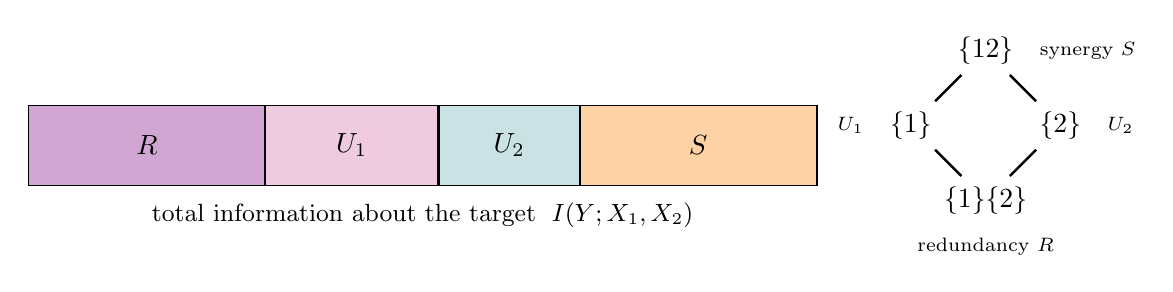
\begin{tikzpicture}[line width=0.9pt]
  % decomposition bar
  \draw (0,0) rectangle (10,1);
  \fill[violet!35] (0,0) rectangle (3,1);
  \fill[accent!22] (3,0) rectangle (5.2,1);
  \fill[accent2!22] (5.2,0) rectangle (7,1);
  \fill[orange!35] (7,0) rectangle (10,1);
  \draw (3,0)--(3,1) (5.2,0)--(5.2,1) (7,0)--(7,1);
  \node at (1.5,0.5) {$R$}; \node at (4.1,0.5) {$U_1$};
  \node at (6.1,0.5) {$U_2$}; \node at (8.5,0.5) {$S$};
  \node[below] at (5,-0.1) {\small total information about the target $\;I(Y;X_1,X_2)$};
  % lattice
  \begin{scope}[xshift=11.2cm, yshift=-0.2cm, scale=0.95]
    \node (top) at (1,2) {$\{12\}$};
    \node (l)   at (0,1) {$\{1\}$};
    \node (r)   at (2,1) {$\{2\}$};
    \node (bot) at (1,0) {$\{1\}\{2\}$};
    \draw (bot)--(l)--(top)--(r)--(bot);
    \node[right=2pt of top,font=\scriptsize] {synergy $S$};
    \node[left=2pt of l,font=\scriptsize] {$U_1$};
    \node[right=2pt of r,font=\scriptsize] {$U_2$};
    \node[below=1pt of bot,font=\scriptsize] {redundancy $R$};
  \end{scope}
\end{tikzpicture}
\caption{Left: the four PID atoms partition the total information $I(Y;X_1,X_2)$. Right: the
redundancy lattice of source collections for two inputs; the four atoms sit on its nodes
(bottom = redundancy, middle = unique, top = synergy).}
\end{figure}

The three identities \eqref{eq:pid}--\eqref{eq:pid-consistency} are \emph{four} unknowns in three
equations: one more definition is required, and there is \textbf{no universally agreed choice}.
Defining a redundancy measure $R$ fixes the rest via
\begin{equation}
  U_i=I(Y;X_i)-R,\qquad S=I(Y;X_1,X_2)-I(Y;X_1)-I(Y;X_2)+R = \mathrm{II}+R ,
\end{equation}
which makes precise the slogan \emph{synergy minus redundancy $=$ co-information},
$S-R=-\mathrm{II}(Y;X_1;X_2)$. Several axiomatic redundancy measures exist --- the original
$I_{\min}$ of Williams \& Beer, the broja measure $I_{\cap}^{\mathrm{BROJA}}$ from an optimisation
over consistent joint distributions, and $I_{\mathrm{ccs}}$ (common change in surprisal) ---
agreeing on the two-source case under the Williams--Beer axioms (symmetry, self-redundancy,
monotonicity) but differing for $n\ge3$. PID is an active research front, and is increasingly used
in neuroscience to ask whether two brain regions, neurons, or frequency bands carry
\emph{redundant}, \emph{unique}, or \emph{synergistic} information about a stimulus or behaviour.

%==================================================================
\section{Continuous variables}
%==================================================================
For a density $f(x)$ the \emph{differential entropy} is $h(X)=-\int f\log f\,\dd x$ (which may be
negative and is not coordinate-free), while mutual information $I(X;Y)=h(X)-h(X\mid Y)$ remains
well defined and invariant under smooth invertible maps.

\paragraph{Differential entropy of a Gaussian, derived.}
For $X\sim\mathcal N(0,\sigma^2)$, $f(x)=\frac{1}{\sqrt{2\pi\sigma^2}}e^{-x^2/2\sigma^2}$ so
$-\ln f(x)=\tfrac12\ln(2\pi\sigma^2)+\tfrac{x^2}{2\sigma^2}$. Taking the expectation,
\begin{align}
  h(X)=\E[-\ln f(X)]
   &=\tfrac12\ln(2\pi\sigma^2)+\frac{\E[X^2]}{2\sigma^2}
    =\tfrac12\ln(2\pi\sigma^2)+\tfrac12
    =\tfrac12\ln\!\big(2\pi e\,\sigma^2\big),
\end{align}
using $\E[X^2]=\sigma^2$ (and $\log_2$ replaces $\ln$ to convert nats to bits).

\paragraph{Maximum-entropy distributions, derived.}
Maximise $h[f]=-\int f\ln f\,\dd x$ subject to $\int f\,\dd x=1$ and $\int x^2 f\,\dd x=\sigma^2$.
Form the Lagrangian with multipliers $\lambda_0,\lambda_2$ and take the functional derivative with
respect to $f(x)$:
\begin{equation}
  \frac{\delta}{\delta f}\!\left[-\!\int f\ln f
   +\lambda_0\!\int f+\lambda_2\!\int x^2 f\right]
  =-\ln f(x)-1+\lambda_0+\lambda_2 x^2 \overset{!}{=}0 ,
\end{equation}
so $f^\star(x)=\exp(\lambda_0-1+\lambda_2 x^2)\propto e^{\lambda_2 x^2}$: a Gaussian (with
$\lambda_2<0$). Fixing the two multipliers by the constraints recovers $\mathcal N(0,\sigma^2)$.
Hence \textbf{among all densities of variance $\sigma^2$ the Gaussian maximises differential
entropy}, $h\le\tfrac12\log(2\pi e\sigma^2)$. The same Lagrange recipe gives the exponential
family $f^\star\propto\exp(\sum_k\lambda_kT_k)$ for moment constraints $\E[T_k]$ (e.g.\ the
exponential distribution on $[0,\infty)$ for fixed mean, the uniform on a bounded interval).

\paragraph{The Gaussian channel, derived.}
Let $Y=X+N$ with $N\sim\mathcal N(0,\sigma^2)$ independent of $X$ and power constraint
$\E[X^2]\le P$. \emph{Step 1}: since $Y\mid X$ is just $N$ shifted by the constant $X$, and
differential entropy is shift-invariant, $h(Y\mid X)=h(N)=\tfrac12\log(2\pi e\sigma^2)$. \emph{Step
2}: $I(X;Y)=h(Y)-h(Y\mid X)=h(Y)-\tfrac12\log(2\pi e\sigma^2)$, so we maximise $h(Y)$. \emph{Step
3}: $\Var(Y)=\E[X^2]+\sigma^2\le P+\sigma^2$, and by the maximum-entropy result $h(Y)$ is largest
when $Y$ is Gaussian, i.e.\ when $X$ is Gaussian, giving $h(Y)\le\tfrac12\log(2\pi e(P+\sigma^2))$.
\emph{Step 4}: subtract:
\begin{equation}
  C=\max_{\E[X^2]\le P} I(X;Y)
   =\tfrac12\log\!\big(2\pi e(P+\sigma^2)\big)-\tfrac12\log(2\pi e\sigma^2)
   =\boxed{\;\tfrac12\log\!\Big(1+\tfrac{P}{\sigma^2}\Big).\;}
\end{equation}
For $n$ parallel independent Gaussian channels with noise powers $\sigma_i^2$, maximising
$\sum_i\tfrac12\log(1+P_i/\sigma_i^2)$ under $\sum_iP_i=P$ with a Lagrange multiplier $\nu$ gives the
\textbf{water-filling} solution $P_i=(\nu-\sigma_i^2)^+$: power is poured into the quietest channels
first.

%==================================================================
\section{Data processing, sufficiency, and Fano}
%==================================================================
\begin{theorem}[Data-processing inequality]
If $X\to Y\to Z$ is Markov ($Z\perp X\mid Y$) then $I(X;Z)\le I(X;Y)$.
\end{theorem}
\begin{proof}
$I(X;Y,Z)=I(X;Y)+I(X;Z\mid Y)=I(X;Z)+I(X;Y\mid Z)$; the Markov property kills $I(X;Z\mid Y)$ and
$I(X;Y\mid Z)\ge0$.
\end{proof}
Equality holds iff $Y$ is a \emph{sufficient statistic} for $X$. No processing of $Y$ creates
information about $X$: a downstream neuron cannot recover more about a stimulus than its afferents
deliver.

\begin{theorem}[Fano's inequality]
For any estimator $\hat X=g(Y)$ of $X$ with error probability $P_e=\Pr(\hat X\neq X)$,
\begin{equation}
  H(X\mid Y)\le H_2(P_e)+P_e\log(\abs{\mathcal X}-1).
\end{equation}
\end{theorem}
Fano converts a bound on residual entropy (hence on $I(X;Y)$) into a bound on decoding error,
linking information to achievable read-out accuracy.

%==================================================================
\section{Application: information in neural responses}
%==================================================================
Let $S\sim p(s)$ be a stimulus and $R$ the neural response (spike count, binned spike train, or
continuous feature). The coding quantity of interest is
\begin{equation}
  I(S;R)=\underbrace{H(R)}_{\text{response entropy}}-\underbrace{\E_S[H(R\mid S)]}_{\text{noise entropy}} :
  \label{eq:neural}
\end{equation}
a neuron is informative when responses are \emph{diverse} across stimuli yet \emph{reliable} for
each stimulus.

\paragraph{Direct method and bias.}
Binning time at resolution $\Delta t$ over $L$ bins yields binary words $w\in\{0,1\}^L$. Estimating
the total and noise entropy rates from many stimulus repetitions gives the Strong--de\,Ruyter--%
Bialek estimate $I_{\mathrm{rate}}=H_{\mathrm{tot}}-H_{\mathrm{noise}}$ (bits/s)~\cite{strong1998,borst1999}. Plug-in entropy
estimates are biased; the leading (Miller--Madow / Panzeri--Treves) bias is
\begin{equation}
  \langle \hat I\rangle - I \;\approx\; -\frac{1}{2N\ln2}\left[\sum_{s}\big(\tilde R_s-1\big)-\big(\tilde R-1\big)\right],
\end{equation}
where $\tilde R_s$ is the number of response bins occupied given stimulus $s$ and $\tilde R$ the
number occupied overall: the bias is of order $(\#\text{states})/N$ for $N$ trials, motivating bias
correction (Panzeri--Treves, NSB estimator)~\cite{panzeri2007} or quadratic extrapolation in $1/N$.

\paragraph{Fisher-information lower bound.}
For a continuous parameter $\theta$ (e.g.\ stimulus orientation) encoded by response $r$ with
likelihood $p(r\mid\theta)$, the \textbf{Fisher information}
$J(\theta)=\E\big[(\partial_\theta\log p(r\mid\theta))^2\big]$ bounds any unbiased estimator
through Cram\'er--Rao, $\Var(\hat\theta)\ge1/J(\theta)$. In the Gaussian/large-$N$ regime the mutual
information is captured by
\begin{equation}
  I(\theta;r)\ \gtrsim\ H(\theta)-\tfrac12\,\E_\theta\!\Big[\log\frac{2\pi e}{J(\theta)}\Big],
\end{equation}
the Brunel--Nadal bound~\cite{brunelnadal1998}, tying coding efficiency to the sharpness of tuning
curves ($J\propto (f'(\theta))^2/\text{noise}$).

\paragraph{Populations: synergy and redundancy.}
For a population $\vec r=(r_1,\dots,r_n)$ the PID and interaction information of
Sections~6--7 ask whether neurons are \emph{redundant} (overlapping codes, robust but inefficient),
carry \emph{unique} information, or are \emph{synergistic} (the joint pattern means more than the
parts). \textbf{Noise correlations} --- shared trial-to-trial variability --- can raise or lower
$I(S;\vec r)$ relative to independent neurons depending on their sign relative to the signal
correlations, the central issue in the population-coding literature.

\paragraph{Efficient coding.}
Maximising $I(S;R)$ over the response distribution under metabolic and noise constraints predicts
that optimal neurons should \emph{decorrelate} and \emph{equalise} their outputs (histogram
equalisation, Laughlin 1981) and match their tuning to the stimulus statistics --- the
information-theoretic foundation of the efficient-coding hypothesis~\cite{barlow1961,laughlin1981}.

%==================================================================
\section{Sequences and the asymptotic equipartition property}
%==================================================================
The deep content of information theory appears when we encode \emph{long sequences}. The following
results (the AEP) formalise the idea that, although an alphabet has $\abs{\mathcal X}^n$ possible
sequences, almost all probability concentrates on a much smaller \emph{typical set} of $\approx
2^{nH}$ sequences~\cite{cohen2024,coverthomas}.

\begin{theorem}[Weak AEP]
Let $X_1,\dots,X_n$ be i.i.d.\ copies of $X$. Then
$\;-\tfrac1n\log p(X_1,\dots,X_n)\xrightarrow{\ \mathrm{prob}\ }H(X)$ as $n\to\infty$.
\end{theorem}
\begin{proof}
By independence, $-\tfrac1n\log p(X_1,\dots,X_n)=\tfrac1n\sum_{i=1}^n\big(-\log p(X_i)\big)$, an
average of i.i.d.\ terms with mean $\E[-\log p(X)]=H(X)$. The weak law of large numbers gives
convergence in probability to $H(X)$.
\end{proof}

\begin{definition}[Typical set]
For $\epsilon>0$, $\;T^{(n)}_\epsilon=\big\{x^n\in\mathcal X^n:\ 2^{-n(H+\epsilon)}\le p(x^n)\le
2^{-n(H-\epsilon)}\big\}.$
\end{definition}

\begin{theorem}[Properties of the typical set]\label{thm:aep}
For every $\epsilon>0$ and $n$ large enough:
(i)~$\Pr\!\big(X^n\in T^{(n)}_\epsilon\big)>1-\epsilon$;
(ii)~$\abs{T^{(n)}_\epsilon}\le 2^{n(H+\epsilon)}$;
(iii)~$\abs{T^{(n)}_\epsilon}\ge(1-\epsilon)2^{n(H-\epsilon)}$.
\end{theorem}
\begin{proof}
(i) is the Weak AEP applied to the event defining $T^{(n)}_\epsilon$. (ii): since every $x^n\in
T^{(n)}_\epsilon$ has $p(x^n)\ge 2^{-n(H+\epsilon)}$,
$1\ge\sum_{x^n\in T^{(n)}_\epsilon}p(x^n)\ge\abs{T^{(n)}_\epsilon}\,2^{-n(H+\epsilon)}$, giving the
bound. (iii): by (i), $1-\epsilon<\Pr(T^{(n)}_\epsilon)\le\abs{T^{(n)}_\epsilon}\,2^{-n(H-\epsilon)}$.
\end{proof}
Thus $\approx 2^{nH}$ sequences carry essentially all the probability and can be indexed with
$\approx nH$ bits --- the intuition behind the source-coding theorem below.

%==================================================================
\section{Source coding I: the Kraft--McMillan theorem}
%==================================================================
A symbol code $c:\mathcal X\to\mathcal Y^*$ maps each symbol to a finite string over an alphabet of
size $d=\abs{\mathcal Y}$; it is \emph{uniquely decodable} if distinct messages have distinct
encodings, and \emph{prefix} (instantaneous) if no codeword is a prefix of another.

\begin{theorem}[Kraft--McMillan]\label{thm:kraft}
(1) Any uniquely decodable code with lengths $\ell_x=\abs{c(x)}$ satisfies
$\sum_{x}d^{-\ell_x}\le1$. (2) Conversely, given lengths $(\ell_x)$ with $\sum_x d^{-\ell_x}\le1$,
there exists a \emph{prefix} code with those lengths.
\end{theorem}
\begin{proof}
(1) For any $n$, expand the $n$-th power
$\big(\sum_x d^{-\ell_x}\big)^n=\sum_{x_1,\dots,x_n}d^{-(\ell_{x_1}+\cdots+\ell_{x_n})}
=\sum_{k=1}^{n\ell_{\max}}a(k)\,d^{-k}$, where $a(k)$ counts messages of total encoded length $k$.
Unique decodability means distinct messages give distinct strings, so $a(k)\le d^{k}$ (there are
only $d^k$ strings of length $k$); hence $\big(\sum_x d^{-\ell_x}\big)^n\le n\ell_{\max}$ and, taking
$n$-th roots and $n\to\infty$, $\sum_x d^{-\ell_x}\le1$. (2) Order $\ell_1\le\cdots\le\ell_{m}$ and
set $r_m=\sum_{i<m}d^{-\ell_i}\le1$; let $c(m)$ be the first $\ell_m$ digits of the $d$-ary
expansion of $r_m$. If $c(m)$ were a prefix of $c(n)$ ($m<n$) then $r_n-r_m<d^{-\ell_m}$, yet by
construction $r_n-r_m=\sum_{i=m}^{n-1}d^{-\ell_i}\ge d^{-\ell_m}$ --- a contradiction. So the code is
prefix.
\end{proof}
\begin{corollary}
For any uniquely decodable code there is a prefix code with the same lengths: restricting to prefix
codes costs nothing.
\end{corollary}

%==================================================================
\section{Source coding II: Shannon's first theorem and optimal codes}
%==================================================================
\begin{theorem}[Source-coding bound for symbol codes]\label{thm:src}
For a uniquely decodable $d$-ary code, $\;H_d(X)\le\E\,\abs{c(X)}$, with equality iff
$\ell_x=-\log_d p(x)$.
\end{theorem}
\begin{proof}
Let $\ell_x=\abs{c(x)}$ and $q(x)=d^{-\ell_x}/Z$ with $Z=\sum_{x'}d^{-\ell_{x'}}\le1$ (Kraft). Then
\begin{align}
  \E\,\abs{c(X)}-H_d(X)
  &=\sum_x p(x)\ell_x+\sum_x p(x)\log_d p(x)
   =\sum_x p(x)\log_d\frac{p(x)}{d^{-\ell_x}}\notag\\
  &=\sum_x p(x)\log_d\frac{p(x)}{q(x)}-\log_d Z
   =\KL(p\,\|\,q)-\log_d Z\ \ge\ 0,
\end{align}
since $\KL\ge0$ (Theorem~\ref{thm:gibbs}) and $Z\le1$. Equality forces $p=q$ and $Z=1$, i.e.\
$\ell_x=-\log_d p(x)$.
\end{proof}
The optimum $\ell_x=-\log_d p(x)$ is generally non-integer. Rounding up ($\ell_x=\lceil-\log_d
p(x)\rceil$, the \textbf{Shannon code}) gives $H_d\le\E\abs{c}<H_d+1$, an overhead of up to one
symbol. \textbf{Block coding} removes it: encoding $n$ symbols at once yields
$H_d(X)\le\frac1n\E\abs{c(X^n)}<H_d(X)+\frac1n\xrightarrow{n\to\infty}H_d(X)$ --- \emph{Shannon's
first (source-coding) theorem}. Several constructions are standard~\cite{cohen2024,mackay2003}:
\begin{itemize}[leftmargin=1.5em]
  \item \textbf{Huffman (1952)} --- provably \emph{optimal} prefix code; build the code tree by
  repeatedly merging the two least probable symbols. \emph{Example}: $p=(0.4,0.2,0.2,0.1,0.1)$,
  $H\approx2.12$ bits, Huffman lengths $(2,2,2,3,3)$, $L=2.2$ bits (within $4\%$ of $H$).
  \item \textbf{Shannon (1948)} and \textbf{Fano (1949)} --- near-optimal length assignments from the
  cumulative distribution.
  \item \textbf{Arithmetic / Elias coding} --- encode the \emph{whole message} as a sub-interval of
  $[0,1)$; approaches $H$ without the per-symbol rounding loss and handles adaptive models.
  \item \textbf{Tunstall (1967)} --- a variable-to-fixed dual that maps variable-length source blocks
  to fixed-length codewords.
\end{itemize}

%==================================================================
\section{Channel coding: Shannon's second theorem}
%==================================================================
A \textbf{discrete memoryless channel} (DMC) is a conditional law $p(y\mid x)$ applied
independently to each symbol. Its \textbf{capacity} is
\begin{equation}
  C=\max_{p(x)} I(X;Y)\qquad[\text{bits per channel use}].
\end{equation}
\emph{Examples.} Binary symmetric channel with crossover $f$: $C=1-H_2(f)$ (so $C=1$ at $f=0$,
$C=0$ at $f=\tfrac12$). Binary erasure channel with erasure probability $e$: $C=1-e$.

An $(m,n)$ code maps $m$ messages to length-$n$ inputs and decodes outputs back to messages; its
\textbf{rate} is $\rho=\tfrac{\log m}{n}$ bits/use, and a rate $R$ is \emph{achievable} if codes
exist with $\rho\to R$ and maximal error $\to0$.

\begin{theorem}[Shannon's second theorem]\label{thm:channel}
For a DMC of capacity $C$, a rate $R>0$ is achievable if and only if $R\le C$.
\end{theorem}

\paragraph{Why $C$ (joint-typicality decoding).} Generate a random codebook of i.i.d.\ inputs and
decode $y^n$ to the unique codeword that is \emph{jointly typical} with it. Two facts make this
work for large $n$: of the $\approx 2^{nH(Y)}$ typical outputs, each input is compatible with
$\approx 2^{nH(Y\mid X)}$ of them, so the number of distinguishable inputs --- whose output sets do
not overlap --- is at most
\begin{equation}
  \frac{2^{nH(Y)}}{2^{nH(Y\mid X)}}=2^{n\,(H(Y)-H(Y\mid X))}=2^{nI(X;Y)} ,
\end{equation}
giving a reliable rate of $I(X;Y)\le C$ bits/use. Optimizing the input distribution attains $C$.
\paragraph{Converse (why not more).} If $R>C$, Fano's inequality forces $H(\text{message}\mid Y^n)$
to stay bounded away from $0$, so the decoding-error probability cannot vanish. Capacity is thus the
sharp threshold between reliable and unreliable communication --- the channel analogue of entropy.

%==================================================================
\section{Error-correcting (block linear) codes}
%==================================================================
Shannon's theorem is non-constructive; \emph{coding theory} builds explicit codes approaching $C$.
A binary \textbf{$[n,k]$ linear code} is a $k$-dimensional subspace of $\{0,1\}^n$, specified by a
generator matrix $G$ (encoding $x\mapsto xG$) or a parity-check matrix $H$ (codewords satisfy
$Hc^\top=0$). Its \emph{minimum distance} $d$ (smallest Hamming weight of a nonzero codeword) sets
its power: it corrects up to $\lfloor(d-1)/2\rfloor$ bit errors. The \textbf{Hamming $[7,4]$ code}
($d=3$) encodes $4$ data bits into $7$ and corrects any single-bit error via its syndrome
$Hc^\top$; modern turbo and LDPC codes approach the Shannon limit closely.

%==================================================================
\section{Rate--distortion: lossy compression}
%==================================================================
When a distortion $D$ is tolerable, the minimal rate is the \textbf{rate--distortion function}
\begin{equation}
  R(D)=\min_{p(\hat x\mid x):\,\E[d(X,\hat X)]\le D} I(X;\hat X).
\end{equation}
For a Gaussian source $X\sim\mathcal N(0,\sigma^2)$ under squared error,
$R(D)=\tfrac12\log\frac{\sigma^2}{D}$ for $0\le D\le\sigma^2$ (and $0$ beyond): each halving of
distortion costs half a bit per sample. This is the lossy counterpart of source coding and the
basis of perceptual compression~\cite{coverthomas}.

%==================================================================
\section{A worked neural-coding example}
%==================================================================
A neuron emits a spike count $R$ in a fixed window in response to one of two equally likely stimuli
$s\in\{1,2\}$ with Poisson statistics of means $\lambda_1=2$ and $\lambda_2=6$. Then
$p(r\mid s)=e^{-\lambda_s}\lambda_s^{\,r}/r!$ and $p(r)=\tfrac12[p(r\mid1)+p(r\mid2)]$, and
$I(S;R)=H(R)-\tfrac12\big[H(\mathrm{Pois}(2))+H(\mathrm{Pois}(6))\big]\approx0.6$ bits. A single
count window thus already resolves most of the $1$-bit stimulus identity, the more so the larger the
separation $|\lambda_1-\lambda_2|$ relative to the Poisson noise $\sqrt\lambda$ --- the discrete
analogue of the $d'$/Fisher-information analysis of tuning curves.

\section*{Exercises}
\begin{enumerate}[leftmargin=1.6em]
  \item Prove $H(X)\le\log\abs{\mathcal X}$ directly from Jensen applied to $-\log$.
  \item Give examples where $I(X;Y\mid Z)$ is (a) larger and (b) smaller than $I(X;Y)$ (hint:
  common cause vs.\ XOR).
  \item Compute the capacity of the binary erasure channel with erasure probability $e$.
  \item For independent fair bits $X_1,X_2$ and $Y=X_1\oplus X_2$, compute all four PID atoms and
  verify $S=1$ bit while $I(Y;X_i)=0$.
  \item Derive the Gaussian rate--distortion function $R(D)=\tfrac12\log(\sigma^2/D)$.
  \item Estimate the plug-in entropy bias for $N$ samples on an alphabet of size $m$, and discuss
  when it matters for neural data.
\end{enumerate}

\section{Summary}
Entropy measures uncertainty and sets the compression limit; relative entropy measures model
mismatch; mutual information \eqref{eq:mi} measures shared information; and beyond pairs,
interaction information and the partial information decomposition \eqref{eq:pid} separate
\emph{redundant}, \emph{unique}, and \emph{synergistic} contributions of multiple sources. The
non-negativity of $\KL$ underlies every inequality; data processing and Fano constrain any
read-out. Applied to neurons via \eqref{eq:neural}, with bias correction and the Fisher-information
bound, these tools turn ``how much does a spike train tell us about the world?'' --- and ``do
neurons cooperate or duplicate?'' --- into measurable quantities, and ground the efficient-coding
theory of neural representation.

\begin{thebibliography}{9}
\bibitem{cohen2024} S.~Cohen. \emph{Information Theory.} Lecture notes, Mathematical Institute,
  University of Oxford, Michaelmas Term 2024 (adapted from notes of H.~Oberhauser and H.~Jin).
\bibitem{shannon1948} C.~E.~Shannon. A mathematical theory of communication.
  \emph{Bell Syst.\ Tech.\ J.} \textbf{27}, 1948.
\bibitem{coverthomas} T.~M.~Cover, J.~A.~Thomas. \emph{Elements of Information Theory.}
  2nd ed., Wiley, 2006.
\bibitem{mackay2003} D.~J.~C.~MacKay. \emph{Information Theory, Inference, and Learning
  Algorithms.} Cambridge University Press, 2003.
\bibitem{borst1999} A.~Borst, F.~E.~Theunissen. Information theory and neural coding.
  \emph{Nature Neuroscience} \textbf{2}, 1999.
\bibitem{strong1998} S.~P.~Strong, R.~Koberle, R.~R.~de~Ruyter van Steveninck, W.~Bialek. Entropy
  and information in neural spike trains. \emph{Phys.\ Rev.\ Lett.} \textbf{80}, 1998.
\bibitem{panzeri2007} S.~Panzeri, R.~Senatore, M.~A.~Montemurro, R.~S.~Petersen. Correcting for the
  sampling bias problem in spike train information measures. \emph{J.\ Neurophysiol.} \textbf{98}, 2007.
\bibitem{brunelnadal1998} N.~Brunel, J.-P.~Nadal. Mutual information, Fisher information, and
  population coding. \emph{Neural Computation} \textbf{10}, 1998.
\bibitem{williams2010} P.~L.~Williams, R.~D.~Beer. Nonnegative decomposition of multivariate
  information. \emph{arXiv:1004.2515}, 2010.
\bibitem{barlow1961} H.~B.~Barlow. Possible principles underlying the transformation of sensory
  messages. In \emph{Sensory Communication}, MIT Press, 1961.
\bibitem{laughlin1981} S.~B.~Laughlin. A simple coding procedure enhances a neuron's information
  capacity. \emph{Z.\ Naturforsch.\ C} \textbf{36}, 1981.
\end{thebibliography}

\end{document}
